\section{Data Overview} \label{dataover}

First we wanted to get an overview of the data we have collected. In total we had collected events from about 3.7 million swap events. The distribution of the swap events on different networks is shown below.
\begin{figure}[H]
    \centering
    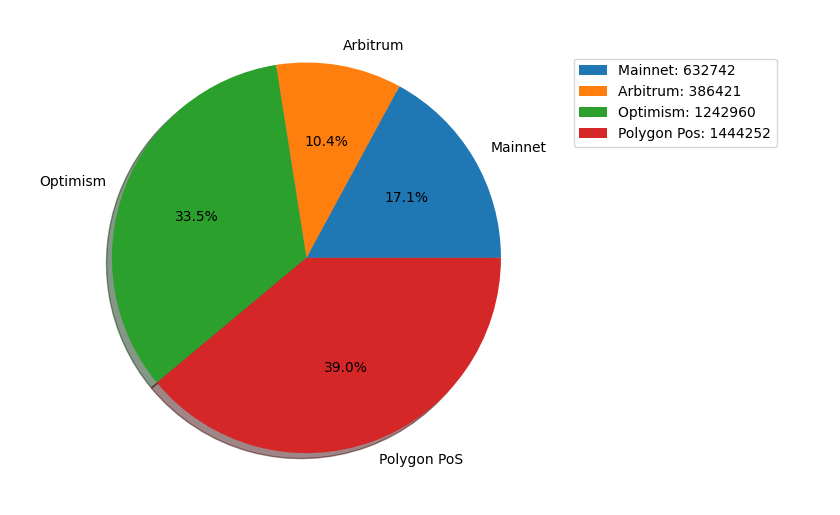
\includegraphics[width=\textwidth]{3_FIGURES/Results/EventDistPlot.PNG}
    \caption{Pie chart of distribution of events on the different networks}
    \label{pieevents}
\end{figure}

A certain number of swap events come from routers. This we assume to mean that the user who made the transaction has used the web-interface that corresponds to the router in question, and is therefore most likely not used to extract cross domain MEV. Below is a table that shows the percentage of swap events initialised by routers belonging to 1inch \cite{1inchprot} or the Uniswap Router:

\begin{table}[h]
\centering
\begin{tabular}{|l|l|l|l|}
\hline
{\color[HTML]{1C1E21} Network}     & {\color[HTML]{1C1E21} All Swap Events} & {\color[HTML]{1C1E21} Non-Router} & Router Percentage \\ \hline
{\color[HTML]{1C1E21} Mainnet}     & {\color[HTML]{1C1E21} 632742}          & {\color[HTML]{1C1E21} 343182}     & 54.24 \%          \\ \hline
{\color[HTML]{1C1E21} Arbitrum}    & {\color[HTML]{1C1E21} 386421}          & {\color[HTML]{1C1E21} 94714}      & 24.51 \%          \\ \hline
{\color[HTML]{1C1E21} Optimism}    & {\color[HTML]{1C1E21} 1242960}         & {\color[HTML]{1C1E21} 556892}     & 44.80 \%          \\ \hline
{\color[HTML]{1C1E21} Polygon PoS} & {\color[HTML]{1C1E21} 1444252}         & {\color[HTML]{1C1E21} 547276}     & 37.89 \%          \\ \hline
{\color[HTML]{1C1E21} Total}       & {\color[HTML]{1C1E21} 3706375}         & {\color[HTML]{1C1E21} 1542064}    & 41.60 \%          \\ \hline
\end{tabular}
\end{table}

As we can see in the table, this drastically reduces the amount of swap events. The remaining events probably originate from other routers, MEV Searchers or other advanced users, though its hard to say for certain. To shed a bit more light on this, we looked at distinct sender addresses. 

\begin{figure}[H]
    \centering
    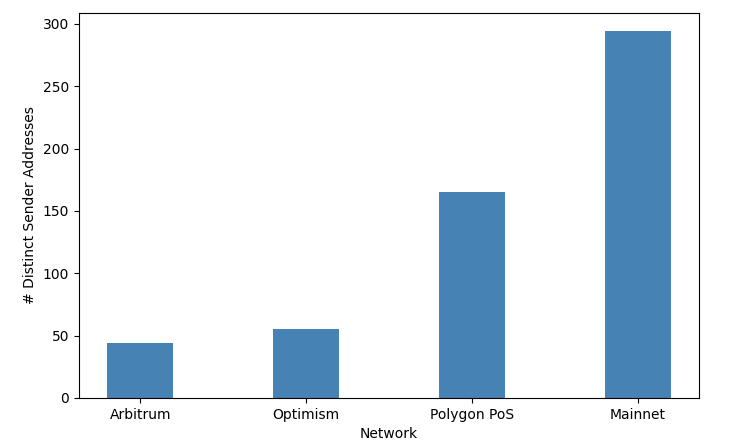
\includegraphics[width=\textwidth]{3_FIGURES/Results/DistinctAddresses.PNG}
    \caption{Bar plot of distinct senders addresses on the different networks}
    \label{bardistintcaddr}
\end{figure}

As seen in \ref{bardistintcaddr}, the amount of distinct addresses is surprisingly low. This is probably because end user would never swap directly against the pool, but use a router. 

\section{First Analysis}

To try and discover cross domain MEV extraction, we first took the union of unique sender addresses of different networks. This yielded new sets of sender addresses that had interacted with Uniswap pools on different networks. The resulting addresses are stored in the appendix \ref{APP:crossaddress}. These addresses were in turn inspected individually using block explores, in order to qualitatively discern whether or not they were engaging in cross domain MEV extraction.

Of the 4 addresses in common between Arbitrum and Optimism, 3 of them seems to be the same MEV searcher deployed to both networks. The final one is doing something with OpenSea, which probably is unrelated to MEV.

For the addresses with Mainnet and Polygon PoS in common, most of them seem to be related to another address, namely 0x0000e0ca771e21bd00057f54a68c30d400000000. These addresses make arbitrages and give the profits to this other address. We are not sure why this is happening, but it looks to be an MEV searcher operating in multiple domains, but not engaging in cross domain MEV.

There are only two addresses that have swapped on both Mainnet and Arbitrum that are not routers. The first one appear to be an MEV searcher that has stopped arbitraging on Mainnet and now does it on Arbitrum instead. The second one is more interesting.
\subsubsection{0xF25d1CeA9772e2584E0A1d4c11AbEa2AEB9B077b}
In this address' transactions we found some cross domain arbitrages

\begin{figure}[H]
    \centering
    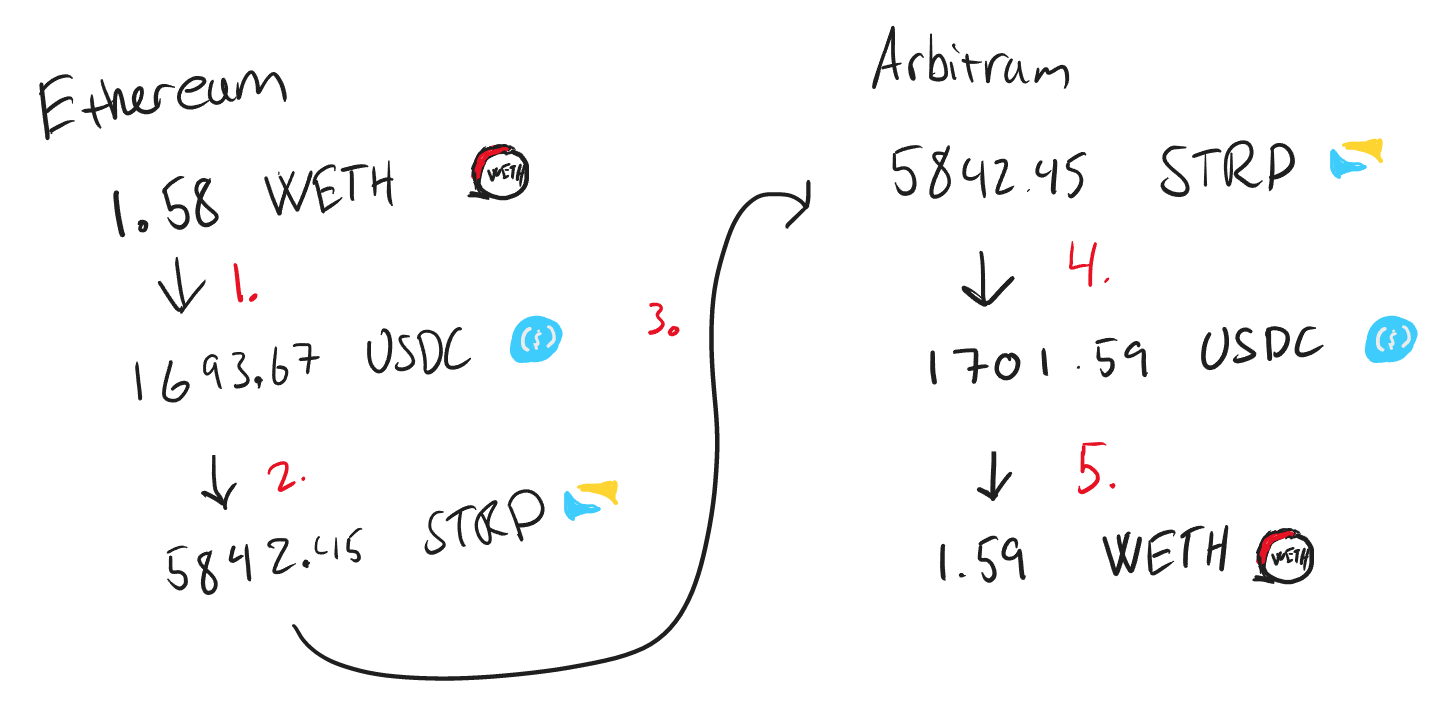
\includegraphics[width=\textwidth]{3_FIGURES/Results/CDMEV.PNG}
    \caption{Example of cross domain arbitrage}
    \label{cdmev}
\end{figure}

Lets go through an example, as visualised in \ref{cdmev}.
\begin{enumerate}
    \item The contract swaps 1.58 WETH for 1693.67 USDC on using a Uniswap V3  pool
    \item It then swaps the USDC gained in step 1 for 5842.45 STRP tokens on a different DEX called Sushiswap
    \item Using the Arbitrum bridge, the STRP tokens are transferred to Arbitrum. Later the STRP tokens are transferred from the ERC20 gateway on Arbitrum to the same smart contract address that did the swaps from step 1 and 2.
    \item It then proceeds to swap the STRP tokens to 1701.59 USDC tokens through
    Sushiswap on Arbitrum
    \item  Finally it swaps the USDC tokens for 1.59 WETH tokens.
\end{enumerate}

You can inspect these transaction yourself on etherscan \href{https://etherscan.io/tx/0x609a6c5d7d1a266a06178cf9da546822d1d4c83ab4309c83e03719985e6b792c}{etherscan.io} and \href{https://arbiscan.io/tx/0x9d7d87f32df33202530d988edc879ba755de0e011e0394583577fe2f0be57ff3}{arbiscan} respectively. 
Looking at the other transaction of this address on these public block explorers, we find that they also do cross domain arbitrage with Gnosis Chain (previously xDai) which is another EVM compatible domain. 
We also see that this contract was created less than a month ago, and has less than a thousand transaction across all the domains we found it to be active on. The profit of these transactions seems to be low, around 0.1-0.2 WETH in the cases we manually checked. 

\section{Second Analysis}
For the second analysis, we tried to find swaps for the same amount of a token but on different chains. This was a much wider net to cast, which is why we tried adding different constraints to it.

Firstly we removed all the swap events that had a router address as sender. As illustrated in \ref{dataover} this almost halves the amount of swap events to consider. But there were too many hits still. The ones we checked were from Swaps of a round number (think 100 or 1000) of USDT, USDC or DAI tokens to any of the other tokens we were tracking. 

In order to reduce the the amount of these types of matches, we tried adding a temporal dimension, such that only swap events that happened within about an hour from each other on different chains would be a match. In order to facilitate this, we needed to timestamp the swap events. This data was not a part of the \texttt{get\_eventLogs} API method that we used to get them, so we had to come up with something else.

The event logs contained metadata about the transactions that emitted them. To place the events temporally, we used the fact that one of these pieces of metadata was the block number of the block that the transaction was included in. Using this we sampled 1000 blocks from each chain, approximately equally distributed across the time window we were looking for swap events in, in order to find the block times for at most 1 hour away from any given other block. The distribution of timestamps across the sampled blocks looks like this: 
\begin{figure}[H]
    \centering
    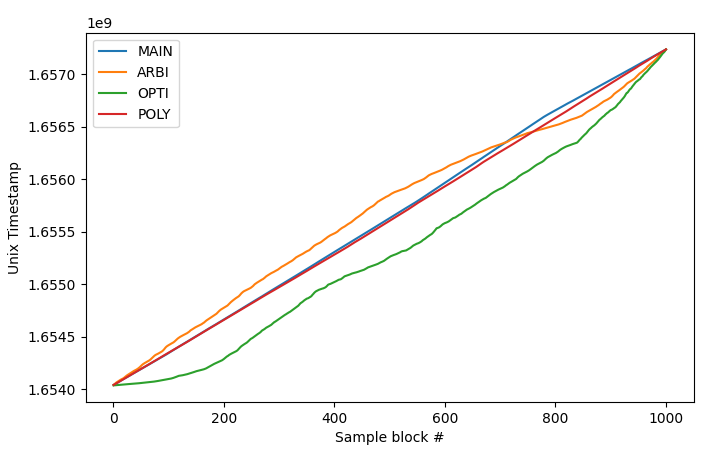
\includegraphics[width=\textwidth]{3_FIGURES/Results/sampleblocktimes.PNG}
    \caption{Unix timestamp of sampled blocks}
    \label{unixtime}
\end{figure}

Adding this criteria did reduce the amount of matches significantly, but there were still too many to manually check. The sample of matches we did check, did not yield anything interesting. They were not temporally close enough or had anything else in common that might suggest they were apart of cross domain arbitrage.

% i tried to do this

% Too many events to check manually

% Maybe if i had access do data (all blokc timestamps) it would be easier

% Need automated classifier to be feasable

% how does one build an automated classifier of cross domain MEV? 
